\newpage
\chapter{Framework Description}
\begin{figure}[t]
    \centering
    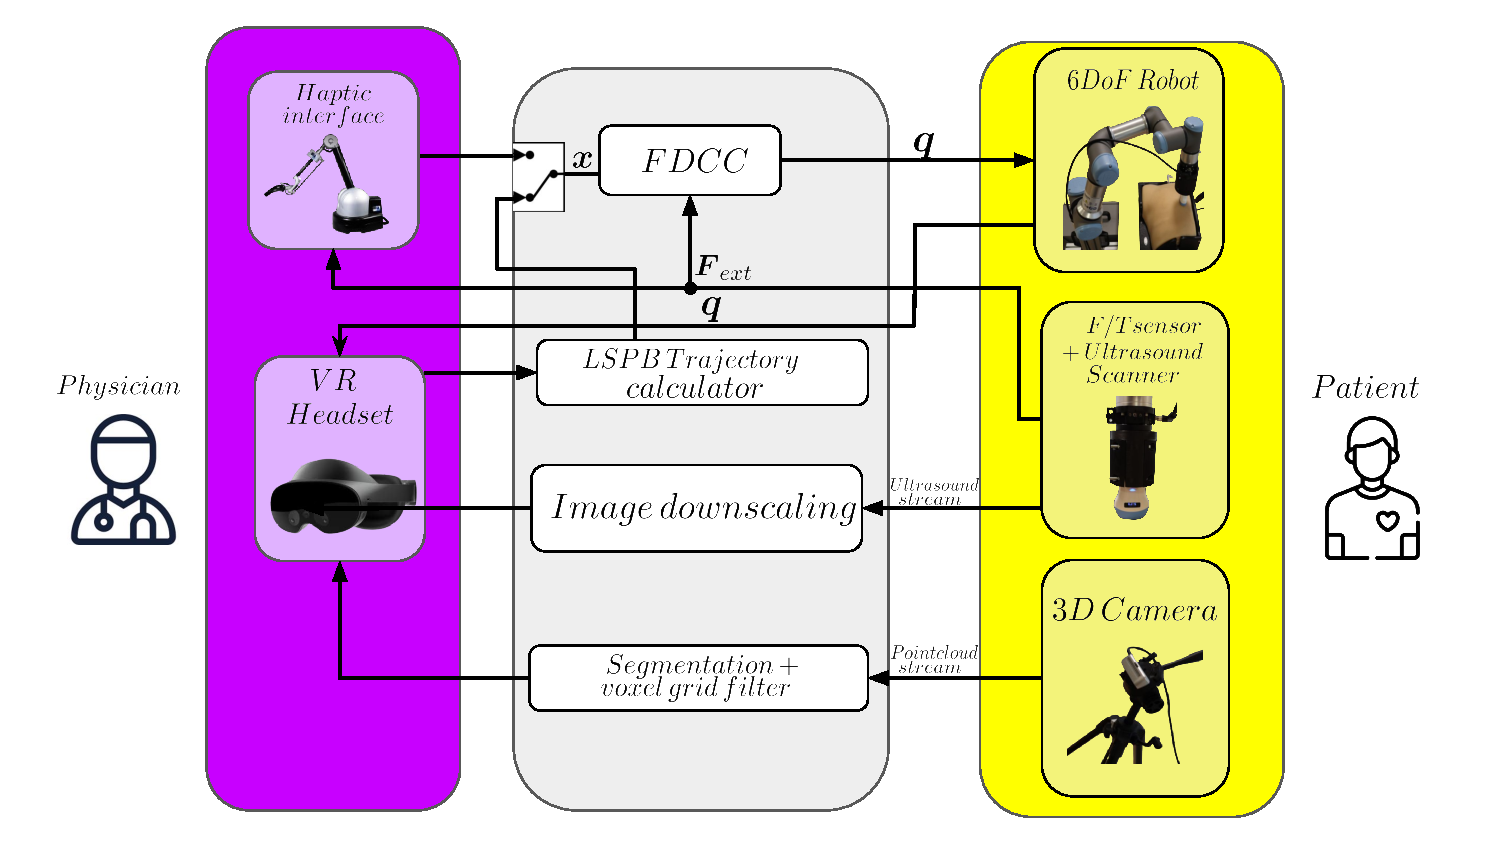
\includegraphics[width=1\columnwidth]{images/framework/framework.pdf}
    \caption{The proposed framework: the physician can teleoperate with the haptic interface or with the waypoint placing method. The visual signals coming from the sensors in the follower's setup are rendered into the VR headset while the force and wrenches feedback are used as input of haptic interface.} 
    \label{fig:framework}
\end{figure}

The remote robotised US framework consists of two main parts: the leader's side, which corresponds to the environment for the physician, and the follower's side, which corresponds to the environment for the patient (see \autoref{fig:framework}). The leader side profits from a real-time updated virtual reality scene streamed over a VR headset with the incoming feedback from the follower, such as the point cloud rendering of the patient overlapped to its SMPL model, the force and wrenches readings of the force and torque sensor mapped into the haptic interface, and the ultrasound probe stream, while the follower side capitalises on a 6Dof robot arm with a force and torque sensor that is controlled with a passive variable Cartesian impedance controller, an ultrasound probe and an RGB-D camera (see \autoref{fig:realenv}).

\subsection{Leader} 
% The leader part of this work is composed by three parts: the haptic interface, the virtual environment and the streaming of the output of the ultrasound probe. 
The haptic interface is the input device that the physician uses to control the relative position and orientation of the robot in real-time. It is controlled with a standard impedance control. We mapped the positions as follows:
\begin{equation}
\boldsymbol{P}^E_{des} = \boldsymbol{P}^E_{start} + \lambda(\boldsymbol{P}^H_{cur} - \boldsymbol{P}^H_{start})
\end{equation}
where $\boldsymbol{P}^E_{des}$ and $\boldsymbol{P}^E_{start}$ $\in \mathbb{R}^{m}$ are respectively the desired and starting position of the end effector, $\boldsymbol{P}^H_{cur}$ and $\boldsymbol{P}^H_{start}$ $\in \mathbb{R}^{m}$ are the current and starting position of the haptic interface, and $\lambda$ $\in \mathbb{R}^{m \times m}$ is a diagonal matrix scaling factor.
For the orientation representation, we used unit quaternions, which are well known to be computationally efficient and singularity-free. We implemented orientation mapping with unit quaternions in the following way:
\begin{equation}
\mathcal{Q}^H_{diff} = \overline{\mathcal{Q}}^H_{cur} * \mathcal{Q}^H_{start}
\end{equation}
\begin{equation}
\mathcal{Q}^E_{des} =\overline{\mathcal{Q}}^H_{diff} * \mathcal{Q}^E_{start}
\label{eq:q_des}
\end{equation}
where $\mathcal{Q}^H_{diff}\in \mathbb{R}^4$ is the relative orientation of the haptic interface with respect to its starting position, $\mathcal{Q}^H_{start}\in \mathbb{R}^4$ and $\overline{\mathcal{Q}}^H_{cur} \in \mathbb{R}^4$ are the starting and the conjugate of the current orientation of the haptic interface, $\mathcal{Q}^E_{des}\in \mathbb{R}^4$ is the desired orientation of the end effector, $\overline{\mathcal{Q}}^H_{diff}\in \mathbb{R}^4$ is the conjugate of $\mathcal{Q}^H_{diff}$ and  $\mathcal{Q}^E_{start}$ is the starting orientation of the end effector. The absence of the scaling factor in \eqref{eq:q_des} is motivated by the fact that we experienced a counterintuitive orientation control if we scale $\overline{\mathcal{Q}}^H_{diff}$.
%In this case, we avoided using a scaling factor because the rotation control seemed to become counterintuitive but it can be achieved anyway using the \verb|Slerp| function, which performs the spherical linear interpolation between quaternions and it is provided in many libraries such as Eigen. \\
At this point, a doctor would already be able to control the robot manipulator and receive force feedback from the patient, but he would miss the visual context of the operation. For this purpose, we recreated the room for ultrasonography in virtual reality (see  \autoref{fig:vrenv}), that can be explored through a VR headset.
We displayed the robot state by applying the joint values to a virtual model, which is visible to the physician. The point cloud computed from the RGBD sensor in the follower framework is rendered over the SMPL model, which is used just to monitor the patient pose. In our virtual scene, we also added a screen for broadcasting the ultrasound image. This feature can exploit VR capabilities to address the problem of not having the patient and the output of the ultrasonography in the same field of view since we can move the screen near the patient or make it follow the headset orientation in a dynamic way. This means that the physician will always be able to monitor both the patient and the ultrasound output, enhancing the control and safety of the teleoperation.
Another consequence related to the use of a virtual environment is the possibility for the doctor to move without limitations around the virtual patient, avoiding constraints on motion due to objects or the patient itself.

\begin{figure}[t]
    \centering
    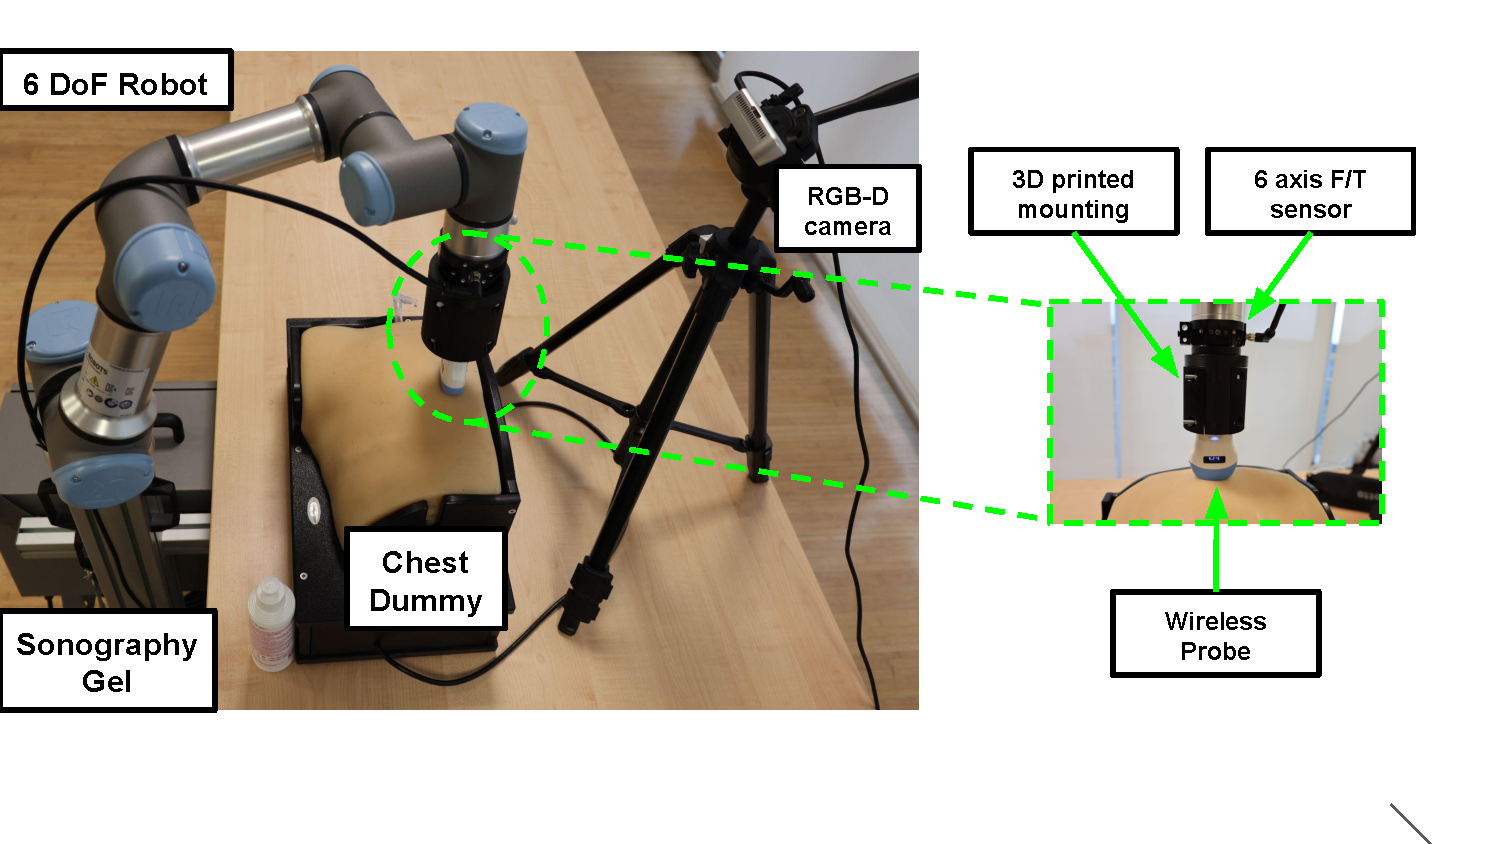
\includegraphics[clip,trim=0 50 0 20, width=1\columnwidth]{images/framework/setup.pdf}
    \caption{In the follower's setup, a chest dummy is used for the examination done by a robot manipulator equipped with a force/torque sensor and an ultrasound probe. A RGBD camera captures the 3d scene, creating a pointcloud.}
    \label{fig:realenv}
    % \vspace{-3mm}
\end{figure}


\begin{figure}[t]
    \centering
    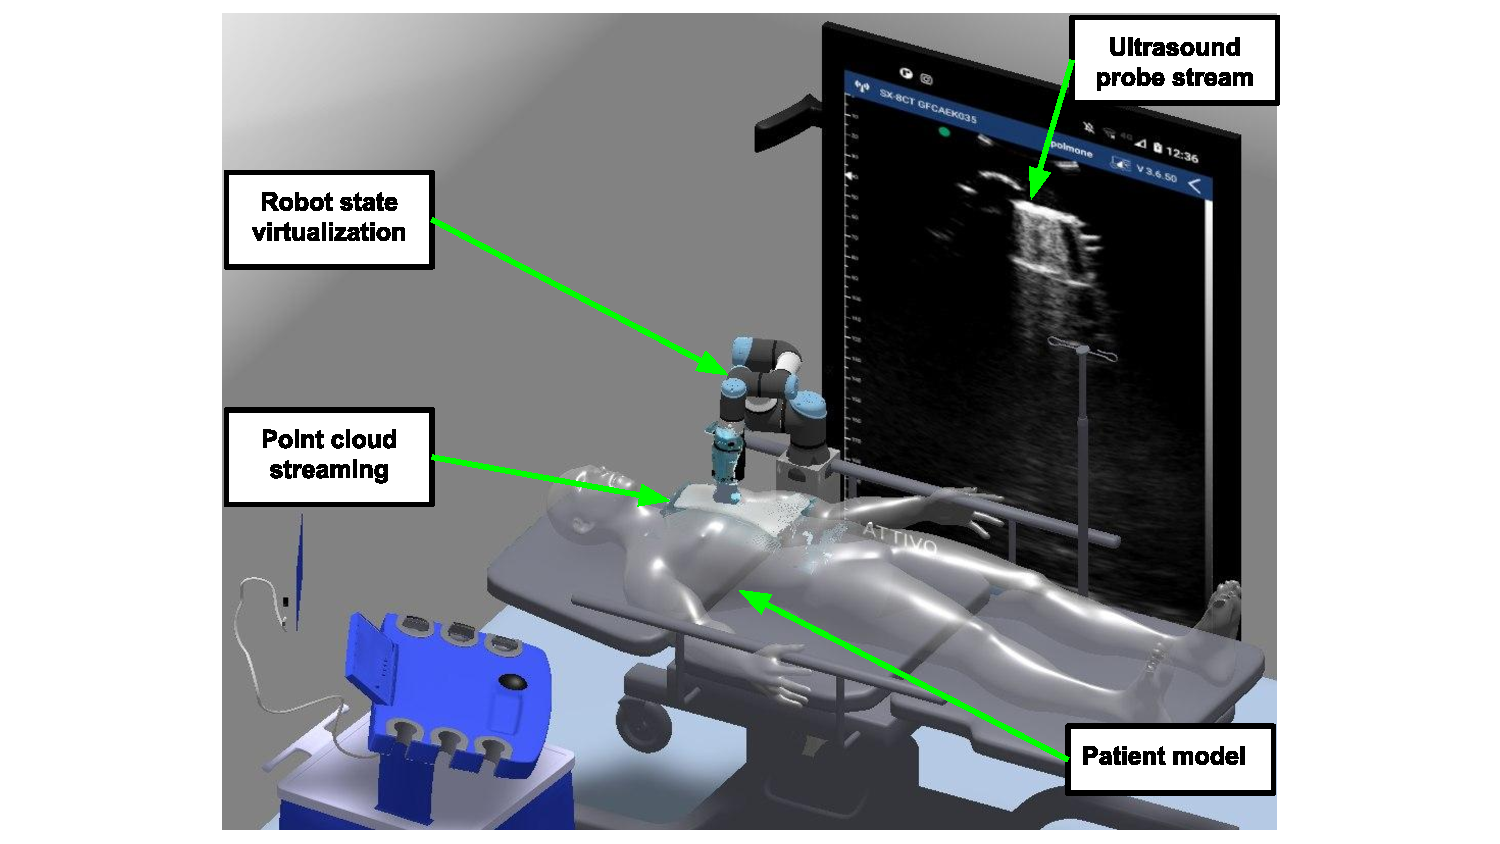
\includegraphics[width=0.9\columnwidth,trim={3.2cm 0 3.2cm 0},clip]{images/framework/env2.pdf}
    \caption{The virtual scene seen by the physician: the pointcloud of the chest dummy is mapped in the same relative pose of the patient's chest, and the stream of the ultrasound probe is put right in front of the physician's view as long as the robot is a digital twin.}
    \label{fig:vrenv}
    % \vspace{-3mm}
\end{figure}


%%%%%%%%%%%%%%%%%%%%%%%%%%%%%%%%%%%%%%%%%%%%
%%%%%%%%%%%%%%%%%%%%%%%%%%%%%%%%%%%%%%%%%%%%
\subsection{Follower}
For the robot's controller, we used the FDCC controller\cite{scherzinger2017forward}, where the closed-loop behaviour of a Cartesian compliant controller relates the external wrenches applied to the end-effector of the robot to a mass-spring-damper model as follows:
%is based on a mass-spring-damper model:
\begin{equation}
\boldsymbol{F}^{ext} = \boldsymbol{\Lambda}^d\ddot{\Tilde{\boldsymbol{x}}} + \boldsymbol{D}^d\dot{\Tilde{\boldsymbol{x}}} + \boldsymbol{K}^d\Tilde{\boldsymbol{x}},
    \label{eq:cartesian_impedance_inertia_shaping}
\end{equation}
where $\Tilde{\boldsymbol{x}} = \boldsymbol{x} - \boldsymbol{x}_d \in\mathbb{R}^{m}$ is the Cartesian error computed with respect to the desired Cartesian end-effector pose $\boldsymbol{x}_d$, $\boldsymbol{F}^{ext}\in\mathbb{R}^{m}$ is the external wrench applied on the end-effector, and $\boldsymbol{\Lambda}_d, \boldsymbol{D}_d ,\boldsymbol{K}_d\in\mathbb{R}^{m\times m}$ are the desired Cartesian inertia, damping, and stiffness, respectively. %The dynamics of this system is based on a mass-spring-damper model.

As system stability might be violated in the presence of a variable impedance controller, we enforced system passivity through the concept of passivity of the power port $\dot{\boldsymbol{x}}^T\boldsymbol{F}^{ext}$.
To do so, we introduce the formalism of port-Hamiltonian systems to describe the interaction model of the variable Cartesian impedance augmented with an energy tank~\cite{ferraguti2015energy} with dynamics:
\begin{equation}
    \dot{\textrm{x}}_t = \frac{\sigma}{\textrm{x}_t}\dot{\Tilde{\boldsymbol{x}}}^T\boldsymbol{D}^d\dot{\Tilde{\boldsymbol{x}}} - \frac{\boldsymbol{w}^T}{\textrm{x}_t}\dot{\Tilde{\boldsymbol{x}}},
\end{equation}
where $\textrm{x}_t \in \mathbb{R}$ is the state of the tank, $\sigma \in \{0,1\}$ modulates the energy storage, and $\boldsymbol{w}$ an the extra input of the port-Hamiltonian system defined as:
\begin{equation} \label{eq:variable_stiffness}
    \boldsymbol{w}(t) = \begin{cases} -\boldsymbol{K}^v(t)\Tilde{\boldsymbol{x}} & \mbox{if $T(\textrm{x}_t)>T_{min}$}  \\ 0 & \mbox{otherwise,} \end{cases}
\end{equation}
where $\boldsymbol{K}^v(t)$ is time-varying component of the stiffness
($\boldsymbol{K}^d(t) = \boldsymbol{K}^{min} + \boldsymbol{K}^v(t)$).
At each time instant, the tank's energy is defined by
$T(\textrm{x}_t)=\frac{1}{2}\textrm{x}_t^2$ and
$T_{min}\in\mathbb{R}^+$ is the minimum energy that the tank is
allowed to store. Thanks to~\eqref{eq:variable_stiffness}, we can
infer the condition $T(\textrm{x}_t)>T_{min}$ when the stiffness is
allowed to raise without violating the passivity constraint. However,
this bound does not prevent the energy of the tank to be drained
instantaneously, situation which leads to the complete loss of
performance. For this reason, it is reasonable to further constrain
the power flow of the tank when the energy is extracted from the tank
($\dot{T}(\textrm{x}_t) > - \eta \nonumber$), where
$\eta\in\mathbb{R}^+$ is the maximum allowed power.
The goal is to track a constant force $\boldsymbol{F}^d$ changing the stiffness matrix, which can be computed solving the QP in ~\eqref{eq:general_QP_formulation}. The optimisation problem involves a trade-off between the precise tracking of a desired wrench and the necessity to uphold a limited level of stiffness.
Inspired by~\cite{zhao2022hybrid}, we formulated the QP as follows:
\begin{align}
    \min_{\substack{\boldsymbol{K}^d \in \mathbb{R}^{m \times m} }} \: & \frac{1}{2} \left( \| \boldsymbol{F}^{ext} - \boldsymbol{F}^{d} \|_{\boldsymbol{Q}}^2 + \| \boldsymbol{K}^{d} - \boldsymbol{K}^{min} \|_{\boldsymbol{R}}^2 \right) \nonumber \\ 
    \quad  \text{s.t.   } \boldsymbol{K}^{min} &\le \boldsymbol{K}^d \le \boldsymbol{K}^{max} \nonumber \\
    \boldsymbol{F}^{min} &\le \boldsymbol{F}^{ext} \le \boldsymbol{F}^{max} \label{eq:general_QP_formulation} \\
    - \boldsymbol{K}^d \Tilde{x} &\leq \sigma \dot{\Tilde{\boldsymbol{x}}}^T \boldsymbol{D}^d \dot{\Tilde{\boldsymbol{x}}} - \Tilde{\boldsymbol{x}}^T 
    \boldsymbol{K}_{min} \dot{\Tilde{x}} + \frac{ T_{t-1} - T_{min}}{\Delta t} \nonumber \\
     %& T(\textrm{x}_t) \ge T_{min} \nonumber \\
    - \boldsymbol{K}^d \Tilde{x} &\leq \sigma \dot{\Tilde{\boldsymbol{x}}}^T \boldsymbol{D}^d \dot{\Tilde{\boldsymbol{x}}} - \Tilde{\boldsymbol{x}}^T 
    \boldsymbol{K}_{min} \dot{\Tilde{x}} - \eta \nonumber
   % & \dot{T}(\textrm{x}_t) \ge - \eta \nonumber
\end{align}
where $N$ is the length of the time window, $\boldsymbol{Q}$ and $\boldsymbol{R}$ $\in \mathbb{R}^{m\times m}$ are diagonal positive definite weighting matrices, $\boldsymbol{K}^d \in \mathbb{R}^{m\times m}$ is the desired stiffness of the Cartesian impedance controller, $\boldsymbol{K}^{min}$ and $\boldsymbol{K}^{max}$ $\in \mathbb{R}^{m\times m}$ are respectively the minimum and maximum allowed stiffness, $\boldsymbol{F}^{ext} \in \mathbb{R}^{m}$ is the wrench of the impedance interaction model, which can be modelled with \eqref{eq:cartesian_impedance_inertia_shaping}, $\boldsymbol{F}^d \in \mathbb{R}^{m}$ is the desired interaction wrench and $\boldsymbol{F}^{max}/\boldsymbol{F}^{min} \in \mathbb{R}^{m}$ is the maximum/minimum wrench that the robot can exert. %The constraint inequality between vectors is element-wise.
The last two constraints limit the maximum energy $T_{min}$ which can be injected in the system and the rate $\eta$ at which the energy is injected and are obtained from $T \le T_{min}$ and $\dot{T} \le -\eta$. 
$1/\Delta t$ is the controller frequency. 
When $T \le T_{min}$ is not satisfied, the stiffness decreases to its minimum ($\boldsymbol{K}^d = \boldsymbol{K}^{min}$). 


More details on the QP problem formulation and energy tank constraint definition are available in~\cite{beber2023passive} referring to the VF-CF control law, but assuming the target force fixed to be fixed instead of pre-computed.
The measured force and torque are used for control but also as feedback for the physician through the haptic interface. A straight one-to-one mapping of these quantities from the sensor to the device produces some vibrations on the haptic interface. This is related to the noise in the F/T sensor readings. To address this problem, we added an exponential moving average filter (EWMA) \cite{roberts1959}, which represent a good trade-off between smoothness and introduced delay:
\begin{equation}
    \boldsymbol{F}^{ext}_H = \boldsymbol{\alpha} \boldsymbol{F}^{ext}_{cur} + (\boldsymbol{I} - \boldsymbol{\alpha}) \boldsymbol{F}^{ext}_{old} 
\end{equation}
where $\boldsymbol{F}^{ext}_H \in \mathbb{R}^{m}$ is a vector of forces and torques that are the target output of the haptic device, $\boldsymbol{F}^{ext}_{cur}$ and $\boldsymbol{F}^{ext}_{old} \in \mathbb{R}^{m}$ are the vectors of forces and torques of the current and precedent control loop, $\boldsymbol{I} \in \mathbb{R}^{m \times m}$ is the identity matrix, and $\boldsymbol{\alpha} \in \mathbb{R}^{m \times m}$ is a diagonal matrix of weights.
 


  
